
\section{Aufgabe E2}
Ordnen Sie die Werte den passenden Histogrammen zu:


\begin{center}
\begin{tabular}{cccc}
Nr. & Mittelwert & Median & Standartabweichung\\
\hline
1 & 10 & 6 & 7,9\\
2 & 10 & 8 & 3,7\\
3 & 10 & 10 & 2,2\\
4 & 10 & 10 & 6,1\\
5 & 10 & 10 & 9,2\\
6 & 10 & 11 & 6,2\\
\end{tabular}
\end{center}
\begin{figure}[!htbp]
\centering
\fbox{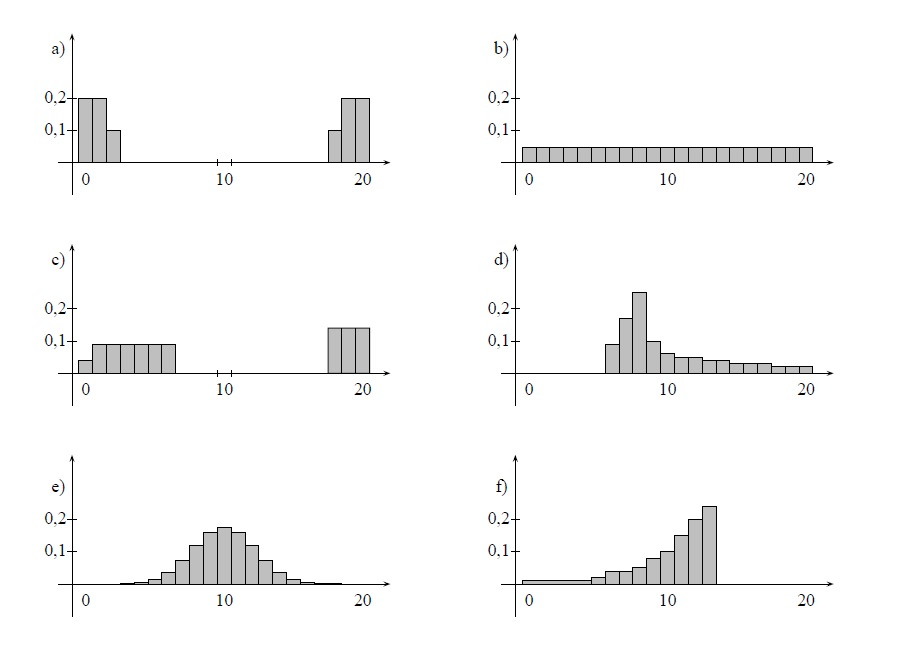
\includegraphics[width=0.9\linewidth]{./chapters/Grafiken_TB/TB_E2.jpg}}
\end{figure}
\newpage

\underline{L�sung:}
\begin{center}
\begin{tabular}{cccc}
Nr. & Mittelwert & Median & Standartabweichung\\
\hline
a) & 10 & 10 & 9,2\\
b) & 10 & 10 & 6,1\\
c) & 10 & 6 & 7,9\\
d) & 10 & 8 & 3,7\\
e) & 10 & 10 & 2,2\\
f) & 10 & 11 & 3,2\\
\end{tabular}
\end{center}


